\chapter{Instructions for Graders}
This details the tasks which should be performed by day-of graders.
Most graders will only need to read this chapter of the manual,
and maybe the terminology section (Appendix~\ref{ch:terms}).

The two functions that you care about are ``Grade Scans''
and ``Classical Grader''

\section{Scan grading}
This is pretty self-explanatory.

\begin{center}
	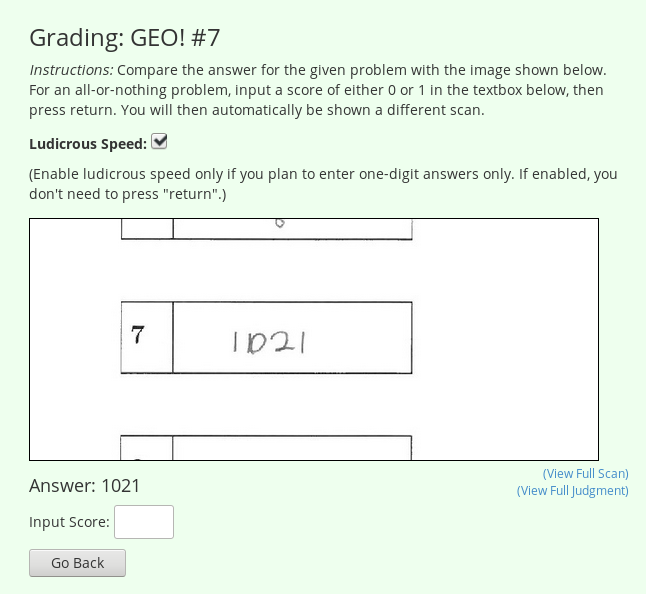
\includegraphics[width=0.8\textwidth]{images/scangrade.png}
\end{center}

%To do this, you should select a problem from the landing page,
%which will open the scan grader for that page.
\begin{itemize}
	\ii Try to select one of the $10$ problems from an exam at random,
	so that we don't end up with everyone problem $1$ or something.
	\ii For all-or-nothing problems,
	type $0$ for an incorrect answer and $1$ for a correct answer.
	\ii Press ``go back'' if you made a mistake and want to fix it.
\end{itemize}
It's possible that you might have some problems
where scores entered are not just $0$ or $1$.
That's fine too.

The option ``ludicrous speed'' is enabled by default (checkbox above),
as long as the problem you are grading is all-or-nothing.
This means that you don't have to press enter.
If you prefer to take things more slowly,
or for some reason the problem you are grading accepts
scores other than $0$ or $1$,
you should disable this option.

If configured, the background of the page may be tinted
with the color of the test, so that you don't accidentally grade
the wrong test.

Towards the end of the stack for a problem,
you may see the same answer several times
(due to latency between submitting a score
and having it saved into the database). This is normal.

\section{Classical grader}
Most importantly:
\emph{do not use the classical grader on problems graded by scan}!
(The interface disables this by default.)

\begin{center}
	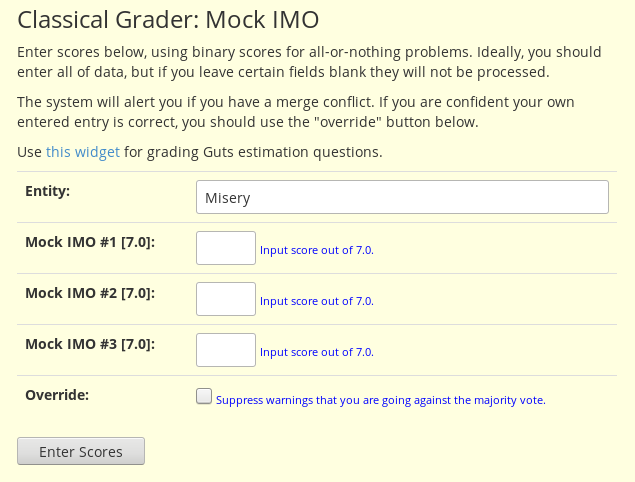
\includegraphics[width=0.8\textwidth]{images/classicgrade.png}
\end{center}

Use the classical grader for tests which are not graded by scan
(for example, the Guts round).
There are two ways you can do this:
\begin{itemize}
	\ii Grade by exam, meaning you are grading many problems on that exam.
	\ii Grade by problem, meaning that you are only grading 
	a particular problem (for example a February proof-based team round problem).
\end{itemize}
Afterwards, this is self-explanatory;
select the entity you want, enter their scores, and submit!

This time, Helium will warn you if you are submitting
a score that goes against a consensus for that problem
(for example if Alice enters 1 and then Bob tries to enter 0 later,
Helium will warn Bob).
If you are confident you are correct, you can use the override option.
However ideally when this happens you should find the person
who submitted the wrong answer before and check with them first.

Whenever you select an entity,
the scores you previously entered for that
entity will be automatically displayed.

If configured, the background of the page may be tinted
with the color of the test, so that you don't accidentally grade
the wrong test.

\section{Matching names}
The other option you can do, if you want something a little
less thoughtless than pressing the zero or one key,
is to help with matching students to names.
This feels quite similar to the scan grader,
but the difference is there are three options you can choose
for each scan.

\begin{center}
	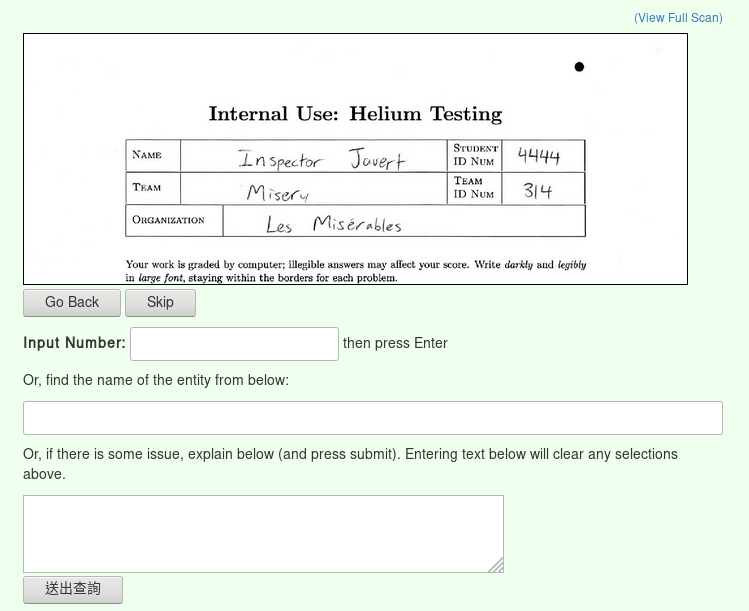
\includegraphics[width=0.7\textwidth]{images/fastmatch2.png}
\end{center}

There are three things you can do for each student name:
\begin{enumerate}
	\ii Most easily, input the student's ID number.
	Type in the student's number into the text box;
	the autocomplete field will then match with the name of the student.
	Press enter to submit.

	\ii Alternatively you can try searching by name.
	Type in the name in the autocomplete field;
	upon getting a match, select it and press enter.
	This works equally well.
	I think it's faster to use ID numbers when possible, but to each their own.

	\ii If their some other issue with the scan
	(e.g.\ there is no name or number at all,
	or the student doesn't appear to exist),
	you should flag it for administrative attention.
	To do this, simply fill in the text box, and press submit.
	An administrator will then be able to deal with it.
\end{enumerate}

\section{Viewing Full Scans, and Broken Scans}
\label{sec:view_full}
When doing scan grading, you can press ``view full page''
in order to see the entire scanned page instead of just the cut-out.
Just click the ``(View Full Scan)'' button near the corner of the image.

Sometimes the scan will have some serious issue with it
(for example, it is blank, or rotated, or illegible, etc.).
If so, then fill out the text box at the top of the page
describing the issue (e.g.\ ``scan is upside down'') and submit it.
This will flag the page for administrative attention, meaning:
\begin{itemize}
	\ii It will no longer appear for any other grader to see.
	\ii It goes in a special queue for officers with the reason you provide.
\end{itemize}

\textbf{Use this feature only if something is wrong with the scan as a whole},
like a missing name or a rotated page.
If it is just an issue with a single problem
(e.g.\ you can't read the student's handwriting on problem three),
just use your best judgement.
Helium has strong conflict resolution; you needn't worry about it yourself.

\section{Guts round}
\begin{itemize}
	\ii Guts round scoring is done using the classical grader.
	\ii For the ``estimation problems'' you will have to compute the score
	to assign to the problems at the end.
	So a ``Guts estimation calculator'', self-explanatory,
	has been provided.
	\ii The old Babbage Guts scoreboard should still be working
	(it now pulls data from Helium).
\end{itemize}

\section{Viewing conflicts}
You can see any evidences you submitted which conflicted with other graders
by pressing ``View Your Grading Conflicts''.
This allows you to also open any particular verdict,
and change your decision on it.

\begin{center}
	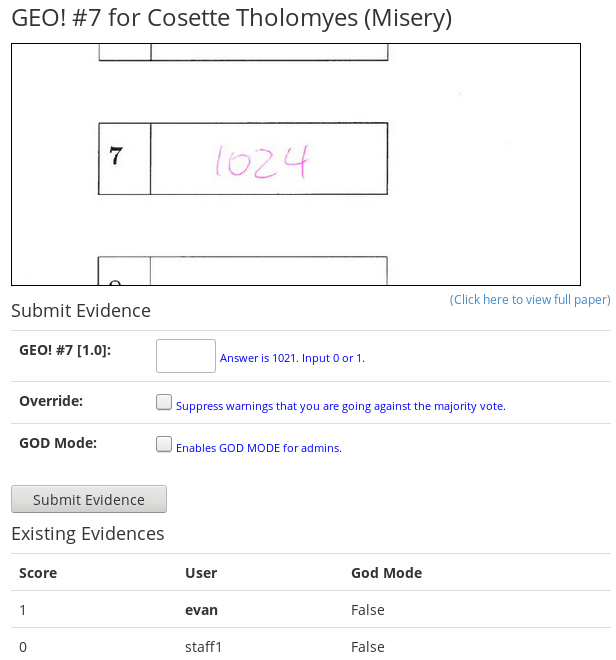
\includegraphics[width=0.7\textwidth]{images/viewverdict.png}
\end{center}
\begin{center}
	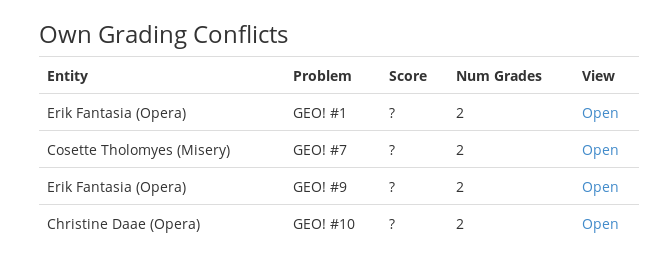
\includegraphics[width=0.8\textwidth]{images/viewconflict.png}
\end{center}

This shouldn't really be necessary for scan grading,
because verdicts are settled with a sufficiently large majority vote anyways.
That is, if you mis-grade a scan, it will eventually sort itself out.

\section{Progress grading}
There are some progress reports on how far grading is going for each problem.
You can use this if you're not sure which problems needs more help.
(Officers may also use this so they can panic as they see things aren't getting done,
or something like that.)

\begin{center}
	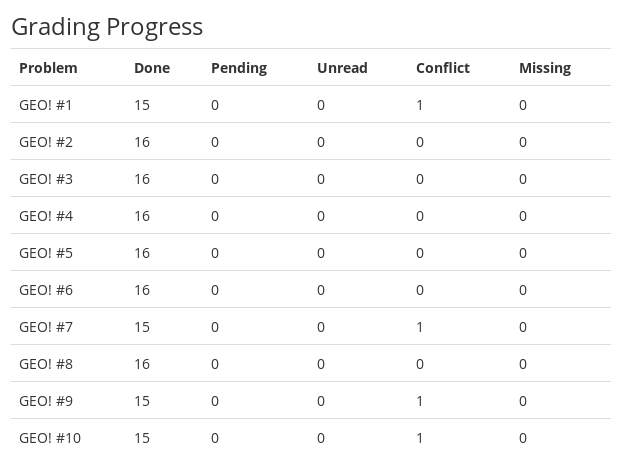
\includegraphics[width=0.8\textwidth]{images/progress.png}
\end{center}


\section{Sneak peek at results}
Some of you may be curious at how teams or students are doing.
While I can't endorse this, the interface lets you do so:
you can poke around the results page,
or look up student papers, etc.
If you do look through this, note that:
\begin{itemize}
	\ii Nothing you see is final, and
	\ii All results are confidential.
\end{itemize}
Note that results are not computed in realtime.
The algorithmic scoring always takes a few minutes.

\section{Do not use ``Upload Scans''}
Unless instructed to do so.
